\documentclass{article}
\usepackage[dvipsnames]{xcolor}
\usepackage[paperwidth=20cm, paperheight=4.5cm, margin = 0cm, top=0.5cm]{geometry}

\usepackage{amsmath}
\usepackage{pgf}
\usepackage{tikz}
\usetikzlibrary{arrows,automata}
\usetikzlibrary{positioning}

\tikzstyle{source}  = [draw,circle,fill=black,thick,inner sep=0mm,minimum size=2mm]

\begin{document}
\begin{center}
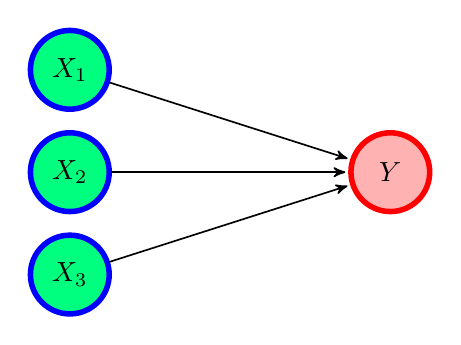
\begin{tikzpicture}[->,>=stealth',shorten >=1pt,auto,node distance=1.3cm,semithick]
                    

\node[state, fill=SpringGreen, draw=blue, line width=2pt, minimum size=1cm] (X1) {$X_{1}$};                   
\node[state, fill=SpringGreen, draw=blue, line width=2pt, minimum size=1cm] (X2) [below of=X1] {$X_{2}$};                   
\node[state, fill=SpringGreen, draw=blue, line width=2pt, minimum size=1cm] (X3) [below of=X2] {$X_{3}$};                   
\node[state, fill=red, opacity = 0.3, draw opacity=1,  draw=red, line width=2pt, text opacity =1, minimum size=1cm] 
(Y) [right = 3cm of X2] {$Y$}       ;                   

\path
	(X1) edge node {} (Y)
	(X2) edge node {} (Y)
	(X3) edge node {} (Y)
	;

\end{tikzpicture}
\end{center}

\end{document}
